\documentclass{article}
\usepackage{amsmath,amssymb,array}
\usepackage{tikz-cd}
\usepackage[hidelinks]{hyperref}
\hypersetup{pdftitle={The Minks Declaration Language},
  pdfsubject={Phase 1 formal specification, issue 50}}

\title{The Minks Declaration Language\\A Draft Specification}
\author{Minks design notes}
\date{Phase 1, issue \#50}

\newcommand{\ttt}[1]{\texttt{#1}}
\newcommand{\keys}{\operatorname{keys}}
\newcommand{\cl}{\operatorname{cl}}
\newcommand{\proj}{\operatorname{pr}}
\newcommand{\make}{\operatorname{make}}
\newcommand{\rel}{\operatorname{Rel}}
\newcommand{\wf}{\mathsf{wf}}
\newcommand{\checkt}{\mathsf{checks}}

\newcommand{\rdefn}[1]{\hypertarget{rule-#1}{\textsc{#1}}}
\newcommand{\ruse}[1]{\hyperlink{rule-#1}{\textsc{#1}}}

\begin{document}
\maketitle

\section{Overview}

A mixin specifies an increment over given data. Its parameters describe
the inputs and its fields specify the operations, choices or laws to
supply. A structure packs choices into one record over given parameters.
A mixin inherits witnesses as parameters. A structure inherits fields
so that further components can refer to the choices already made.

A declaration $d$ is checked in an environment $\mathcal E$ of Rocq
declarations and registered Minks signatures. Checking computes a
signature $\Sigma$. Generation reads $\Sigma$ and produces Rocq
declarations $D$, hierarchy entries $J$ and registrations $R$:
\[
  d \ \xrightarrow{\ \mathrm{check\ in}\ \mathcal E\ }\ \Sigma
    \ \xrightarrow{\ \mathrm{generate\ in}\ \mathcal E\ }\ (D,J,R).
\]
The next declaration is checked in the updated environment.

\begin{itemize}
\item Section~\ref{sec:language} gives the syntax and scope of the two commands.
\item Section~\ref{sec:wf} states the shared well-formedness judgments. Section~\ref{sec:signatures} computes their result for each command.
\item Section~\ref{sec:generation} derives declarations, views and registrations from that result.
\item Section~\ref{sec:properties} states the proof obligations. Section~\ref{sec:examples} works through the declarations and their rejection cases.
\end{itemize}

\paragraph{Rule index.}
{\small\raggedright
\textit{Checking.} \ruse{WF-Decl}, \ruse{WF-Extends}, \ruse{Args-Check},
\ruse{Input-Name}, \ruse{WF-With}, \ruse{Args-Infer}, \ruse{WF-Omit}, \ruse{Univ-Inst},
\ruse{Struct-Univ}, \ruse{Univ-Assemble}.\par
\textit{Mixin signatures.} \ruse{Mixin-Ext}, \ruse{Parent-Scan},
\ruse{Witness-Share}, \ruse{Binder-Order}, \ruse{Expand-Field}.\par
\textit{Structure signatures.} \ruse{Parent-Union}, \ruse{Ancestor-Agree},
\ruse{Struct-Pack}, \ruse{With-Assembly}, \ruse{Export-Fix},
\ruse{Export-Common}.\par
\textit{Generation.} \ruse{Projection-Name}, \ruse{Parent-To}, \ruse{Parent-Of}, \ruse{Export-Form},
\ruse{Export-To}, \ruse{Export-Of}, \ruse{WF-Compare}, \ruse{View-Match},
\ruse{View-Explicit}, \ruse{Coerce-Parent}, \ruse{Inst-Field},
\ruse{Canon-View}, \ruse{Section-End}.\par
\textit{Proof obligations.} \ruse{Gen-Preserve}, \ruse{Fix-Compose}.\par}

\section{Language and scope}
\label{sec:language}

\subsection{Grammar at a glance}
Angle brackets enclose optional syntax and an overbar denotes a sequence.
Parent arguments are juxtaposed. Lists after \ttt{extends}, \ttt{with}
and \ttt{exports}, and lists inside literal brackets, are comma-separated.
$\Delta$ stands for Rocq parameter binders, $U$ for a universe declaration
and $\iota$ for a universe instance. The sort and field body use Rocq syntax.

\newcommand{\grammarArg}{%
  \mathit{arg} &::=& \mathit{param}\mid \ttt{(}\mathit{formal}\ \ttt{:=}\ \mathit{param}\ttt{)}}
\newcommand{\grammarMixinDecl}{%
  \mathit{mixinDecl} &::=&
 \ttt{Minks.Mixin}\ \mathit{mixin}\langle U\rangle\ \Delta\
 \langle\ttt{extends}\ \overline{\mathit{mixinParent}}\rangle\\
 &&\quad \langle\ttt{:}\ \mathit{sort}\rangle\ \ttt{:=}\ \mathit{body}\ \ttt{.}}
\newcommand{\grammarMixinParent}{%
  \mathit{mixinParent} &::=& \mathit{mixin}\langle\iota\rangle\ \overline{\mathit{arg}}}
\newcommand{\grammarStructDecl}{%
  \mathit{structDecl} &::=&
 \ttt{Minks.Struct}\ \mathit{struct}\langle U\rangle\ \Delta\
 \langle\ttt{extends}\ \overline{\mathit{structParent}}\rangle\\
 &&\quad \langle\ttt{with}\ \overline{\mathit{component}}\rangle\
 \langle\ttt{exports}\ \overline{\mathit{export}}\rangle\ \ttt{.}}
\newcommand{\grammarStructParent}{%
  \mathit{structParent} &::=& \mathit{struct}\langle\iota\rangle\ \overline{\mathit{arg}}
 \mid \mathit{native}\langle\iota\rangle\ \overline{\mathit{arg}}}
\newcommand{\grammarComponent}{%
  \mathit{component} &::=& \mathit{key}\ \langle\ttt{as}\ \mathit{proj}\rangle\
 \ttt{:}\ \mathit{mixin}\langle\iota\rangle\
 \langle\ttt{[}\overline{\mathit{input}}\ttt{]}\rangle}
\newcommand{\grammarInput}{%
  \mathit{input} &::=& \mathit{param}\mid\mathit{key}}
\newcommand{\grammarExport}{%
  \mathit{export} &::=& \mathit{interface}\ \langle\ttt{[}\overline{\mathit{selection}}\ttt{]}\rangle}
\newcommand{\grammarSelection}{%
  \mathit{selection} &::=& \mathit{key}\mid\mathit{struct}}

\[
\begin{array}{@{}rcl@{}}
\grammarMixinDecl\\
\grammarStructDecl\\
\grammarArg\\
\grammarMixinParent\\
\grammarStructParent\\
\grammarComponent\\
\grammarInput\\
\grammarExport\\
\grammarSelection
\end{array}
\]

\subsection{Parameters, fields and keys}

The enclosing Rocq sections and the declaration header $\Delta$ form one
ordinary parameter environment. A parameter may depend on earlier inputs.
Only the declaration's \ttt{extends} clause introduces parents.
A witness is a value of a mixin at particular arguments. A field belongs
to a value of a class or record, and a projection reads it. In a
structure, a \emph{key} identifies a field across inheritance, component
selection and export. Two choices of the same mixin may have different keys.

\[
\begin{array}{@{}rcl@{}}
\grammarArg
\end{array}
\]

Both commands use this argument form in parent applications. Each actual
names an ordinary input in scope. Supply explicit formals by position and
implicit ordinary formals by name. Each argument is checked at the type
determined by the preceding arguments.

\subsection{Mixin declarations}
\label{sec:mixin-app}

\[
\begin{array}{@{}rcl@{}}
\grammarMixinDecl\\
\grammarMixinParent
\end{array}
\]

The header binds the mixin's ordinary inputs. Each parent names a
registered mixin at those inputs. Its inherited witnesses are available
when checking the fields in the body. The optional sort follows the
parent list.

\subsection{Structure declarations}
\label{sec:packing}

\[
\begin{array}{@{}rcl@{}}
\grammarStructDecl
\end{array}
\]

The header binds the structure's external parameters. The clauses list
its parents, its local components and its relative interfaces, in that order.

\paragraph{Parents (\texttt{extends}).}

\[
\begin{array}{@{}rcl@{}}
\grammarStructParent
\end{array}
\]

A registered structure supplies its fields at the given ordinary
arguments. A native Rocq type supplies the one-field parent described
by \ruse{Native-Base}.

\paragraph{Components (\texttt{with}).}

\[
\begin{array}{@{}rcl@{}}
\grammarComponent\\
\grammarInput
\end{array}
\]

A component has a key and a mixin. The optional \ttt{as} names its
projection. An explicit list takes parameters or available fields in
mixin-parameter order. Omitting the brackets requests field inference.

\paragraph{Relative interfaces (\texttt{exports}).}

\[
\begin{array}{@{}rcl@{}}
\grammarExport\\
\grammarSelection
\end{array}
\]

Each entry names an interface. A bracketed list selects field keys and
at most one packed structure to fix. A written \ttt{[]} fixes no fields.
Omitting the brackets selects the common fields of the direct parents
(\ruse{Export-Common}).

\paragraph{Scope of names.}

References resolve in the preceding environment, including visible imports.
An export may refer to the structure being declared. Required names must
be fresh and all required Rocq checks must succeed.

Parent arguments name inputs in scope. General terms, the
\ttt{@Parent} form and automatic synthesis of mathematical evidence are
outside this fragment. Host typing and universe checks are premises.
Hierarchy Builder's factories and builders give a related account of
packed hierarchies \cite{hb}. Minks specifies how to select witnesses
by key and how to expose relative interfaces over those selections.

\section{Well-formedness judgments}
\label{sec:wf}

Scope, substitution and definitional equality $\equiv$ are those of Rocq.
Write $\Gamma\vdash_\Phi t:T$ for host typing under universe constraints
$\Phi$. References use resolved binding identities. In $\Gamma$, let
$P$ be the ordinary parameters and visible section assumptions, and
$F$ the inherited and preceding local fields. A parameter of class type
still belongs to $P$.

\rdefn{WF-Decl}. Write $\Gamma\vdash_\Phi d\Downarrow_{\wf}\Sigma$
when the ordinary parameters and parents check and the command's
formation rules compute $\Sigma$. A mixin checks its body in field order
over the computed binders. A structure checks its parent union and
components, then its exports against the completed layout. A field enters
scope only after it checks. Section~\ref{sec:signatures} defines the two
forms of $\Sigma$.

\subsection{Parent and component arguments}

\rdefn{WF-Extends}. For a parent $H$ with ordinary telescope $\Delta_H$,
substitute the supplied arguments into each subsequent parameter type.
A repeated actual is legal and a closed parent takes the empty substitution.
\[
 \frac{H\ \wf\qquad \Gamma\vdash_\Phi\sigma:\Delta_H
       \qquad\operatorname{im}(\sigma)\subseteq P}
      {\Gamma;P\vdash_\Phi H[\sigma]\ \mathsf{parent}}
\]

\rdefn{Input-Name}. For an explicit name $x$ inside a \ttt{with} input
list, let $P_x$ contain the visible ordinary binder named $x$ after
Rocq scope resolution, if any. Let $F_x$ contain the available field
with key $x$, if any. Resolve the name before checking its expected type:
\[
  \frac{P_x\mathbin{\uplus} F_x=\{r\}}
       {\Gamma;P;F\vdash x\Downarrow r}.
\]
The union distinguishes parameter and field identities. Zero matches give
an unknown name and two give an ambiguity. A projection alias does not
enter $F_x$. This applies to explicit fixed inputs of a virtual mixin
as well. Parent arguments still use $P$ and omitted lists still use $F$.

\rdefn{Args-Check}. Let $\mathsf{args}_\Phi(\Gamma,M,\bar r)$ mean that
$\bar r$ supplies the normalized telescope $(z_j:T_j)_{j=1}^n$ of $M$
at the correct arity, with the required head and argument references at
each witness position and
$\Gamma\vdash_\Phi r_j:T_j[\bar r_{<j}/\bar z_{<j}]$ for every $j$.
The explicit selection judgment is
\[
 \frac{\bar r\in(P\cup F)^n\qquad\mathsf{args}_\Phi(\Gamma,M,\bar r)}
      {\Gamma;P;F\vdash_\Phi M[\bar r]\Downarrow M(\bar r)}
 \quad\text{\rdefn{WF-With}} .
\]
\paragraph{Surface shorthand for \ttt{with}.}
\rdefn{Args-Infer}. An omitted input list expands to a tuple of resolved
field references. At this entry, form the candidate set
$D=\{\bar r\in F^n\mid\exists\Phi'.\
\mathsf{args}_{\Phi\cup\Phi'}(\Gamma,M,\bar r)\}$, where $\Phi'$ is a
legal local extension.
\[
 \frac{D=\{\bar r\}}
      {\Gamma;P;F\vdash_\Phi M[?]\;\leadsto\;M[\bar r]}
 \quad\text{\rdefn{WF-Omit}} .
\]
Uniqueness counts binding tuples. Several universe solutions for the
same tuple give one candidate. Check the expanded application by
\ruse{WF-With} and in the completed declaration, just as for written inputs.

\subsection{Universe constraints}
\label{sec:univ}

\rdefn{Univ-Inst}. Explicit universe binders fix the positional order.
A closed binder must suffice for the declaration. An open binder such
as \verb|@{u v +}| permits additional inferred levels after the named
ones. A reference instantiates the declaration's constraints at its
written or inferred levels. For an unannotated mixin, inferred levels
are generalized under \ttt{Set Universe Polymorphism} and fixed under
\ttt{Unset Universe Polymorphism}.

\rdefn{Struct-Univ}. The packed record and its views are universe-polymorphic.
With no binder, generalize inferred levels and constraints. For the native
parent shorthand, take the native type's local levels in declared order,
unified levels once, followed by the remaining inferred levels.
\rdefn{Univ-Assemble}. Check all parents, merged fields, shared witnesses
and result sorts in one compatible universe context. Distinct uses may
instantiate a polymorphic constant independently. Each selection candidate
is checked with local constraints. Only the selected candidate constrains
the declaration. The generated record, projections, views, exports and
packers must admit every assignment allowed by the checked layout.

\section{Computing the internal signatures}
\label{sec:signatures}
Both signatures retain the declaration name, universe context and direct
parent applications. Their dependent telescopes record where each input
comes from and which later fields may use it.

\subsection{Computing the mixin parameter list}
\label{sec:mixin-parameters}
The input is the child's ordinary header $\Delta=(x_1,\ldots,x_n)$
and its list of checked parent applications. A visible section assumption
is already in scope. The signature retains the ordered binders and their roles, local
definitions assembling exported parents, the sort and the checked fields. References below
are binder identities, including the projection path for a base field.

\rdefn{Mixin-Ext}. Instantiate each ordinary parent at its supplied
arguments. Inherit its witness parameters and its own witness as implicit
parameters. An exported parent expands by \ruse{Expand-Field}. Its
assembled class value is a local definition. Check the Rocq body at the
given or inferred sort over the resulting context. Each subsequent
field may use earlier fields, including their bodies when defined.

\paragraph{Read each parent.}
\rdefn{Parent-Scan}. Start with an empty ordered table $T$ of inherited
binders. For each parent $H$ in source order, start a fresh substitution
$\sigma$ with its checked ordinary arguments (\ruse{WF-Extends}).
Visit the signature of $H$ in order. Write $\mathsf{intern}(d)$ for the
operation below, which updates $T$ and returns a binder identity.
\[
\begin{array}{ll}
 \text{entry in the signature of }H & \text{action}\\ \hline
 z\text{ ordinary} & \text{use the supplied }\sigma(z)\\
 z\text{ a witness of descriptor }d &
       \sigma(z)\gets\mathsf{intern}(d[\sigma])\\
 z:=t & \sigma(z)\gets t[\sigma]
\end{array}
\]
For an ordinary parent, finish by interning its own witness, with head
$H$, absent key, instantiated levels and its full argument list under
$\sigma$. For a virtual parent, traverse the remainder by
\ruse{Expand-Field}, interning each substituted descriptor and binding
its key to the result before the next step. Save the assembled
constructor application as a local definition. Both visits share the
same table across all parents.

\paragraph{Identify repeated occurrences.}
\rdefn{Witness-Share}. A witness descriptor carries a head $M$, an
optional key $k$, ordered references $\bar r$ and universe instance
$\iota$. An ordinary descriptor from an export carries a key and type.
For an incoming descriptor $d$, form $C(d)$ from the entries of $T$:
\[
\begin{aligned}
  k\sim k' &\iff k=k'\ \lor\ k=\bot\ \lor\ k'=\bot,\\
 C(M,k,\bar r,\iota)
   &=\{t\in T_{\rm witness}\mid M_t=M,\ k_t\sim k\},\\
 C(k:\tau)&=\{t\in T_{\rm ordinary}\mid k_t=k\}.
\end{aligned}
\]
Here $\bot$ denotes an absent key. For two witnesses,
$\mathsf{agree}(t,d)$ requires identical ordered references and
compatible instances. Merge instances positionwise: a hole takes its
partner, two holes remain a hole, and two explicit entries must agree.
An omitted instance supplies holes at all positions. For ordinary
entries, agreement is the descriptor compatibility of \ruse{Parent-Union}.
With $h$ a fresh identity, the update is
\[
\begin{array}{lll}
 C(d) & \text{new table} & \text{return}\\ \hline
 \varnothing & T\mathbin{+\!\!+}[(h,d,1)] & h\\
 \{t\},\ \mathsf{agree}(t,d)
     & T[t\gets\mathsf{merge}(t,d)] & h_t\\
 \text{otherwise} & \text{reject} &
\end{array}
\]
Merge retains the position and identity of $t$, adopts any supplied
key and levels, and increments its occurrence count. Thus an unkeyed
occurrence seeing two keyed choices is ambiguous even if filtering by
arguments would leave only one. All later references use the returned
identity.

\paragraph{Emit binders in scope.}
\rdefn{Binder-Order}. Let $j$ be the number of header binders already
emitted, initially zero. Let $U$ be the unprinted entries of $T$.
An entry is ready when every inherited identity referenced by its type
or arguments has been emitted. Among ready entries choose the least
lexicographic rank
\[
  \bigl(\mathbf 1_{\{\mathrm{count}=1\}},\
           \mathrm{first\ occurrence}\bigr).
\]
For the chosen entry $t$, let $b$ be the maximum of $j$ and the
indices of header binders used in its type or argument references.
With $\Delta_{j:b}=(x_{j+1},\ldots,x_b)$, emit recursively:
\[
\begin{aligned}
 \mathsf{emit}(j,\varnothing)&=\Delta_{j:n},\\
 \mathsf{emit}(j,U)&=\Delta_{j:b}\ \cdot\ [t]\ \cdot\
                         \mathsf{emit}(b,U\setminus\{t\}).
\end{aligned}
\]
A nonempty $U$ with no ready entry fails. Header binders retain their
flags; ordinary export entries are explicit and witness entries are
implicit typeclass parameters. Record each witness's head, key, levels
and references at their final positions. Append saved local definitions
in parent order for checking the class body. They occupy no argument
position. Each recursive call consumes one table entry.

\subsection{Computing the structure layout}

A structure layout $A$ is a telescope over the external parameters $\Delta$. A keyed
field $k:T$ records its type and projection annotation. A component
$k:M(\bar r)$ also records its mixin and ordered argument references.
Each reference starts at a parameter or a preceding field, possibly
followed by a registered base projection. These references and the
free local references in ordinary field types determine dependencies.
With $\Gamma_P$ the parameter context and $s$ an admissible result sort:
\[
 \frac{\Gamma_P\ \wf}{\Gamma_P\vdash_\Phi ()\ \wf}
 \qquad
 \frac{\Gamma_P\vdash_\Phi A\ \wf\quad k\notin\keys(A)\quad
       \Gamma_P,A\vdash_\Phi T:s}
      {\Gamma_P\vdash_\Phi (A,k:T)\ \wf}.
\]

\paragraph{Parents.}
\rdefn{Native-Base}. Resolve a registered structure directly. For a
native type head $B$, reuse the visible base registered for its Rocq
identity. On first use, generate $B\ttt{Carrier}$ in the current module
and register it as a Minks structure with no structure parents. Its
parameter telescope is that of $B$. At parameters $\bar x$ it has one
ordinary field $\ttt{carrier}:B\,\bar x$. The sort \ttt{Type} uses
the same rule with an empty telescope and a fresh universe.
Register the base's projection to the native target as a coercion.
Base creation and child generation belong to one declaration transaction.
An occupied generated name or competing visible bases for one head
require an explicit resolution; a name alone cannot identify a base.

\rdefn{Parent-Union}. Apply the resolved parent to the supplied
arguments in the child's context and use its instantiated field layout.
Generation constructs the base record and this application directly.
A child takes the flattened field values in its constructor and obtains
the ordinary \ttt{To} and \ttt{Of} maps for its direct parent.
An empty parent list contributes an empty layout.

Merge inherited fields by key. A shared key must have the same kind of
descriptor, convertible field types and, for mixin fields, the same mixin
and ordered references after substitution. Retain the requested coercions
on the merged projection, subject to Rocq's checks.
\rdefn{Ancestor-Agree}. Along all declared paths to the same qualified
ancestor, the instantiated ancestor types must convert and each ancestor
key must select the same child key. Record one key map per ancestor.
A conflict rejects the declaration, even for an unused ancestor parameter.

\paragraph{Components.}

A direct \ttt{with} entry selects a mixin. A written list supplies its
full parameter telescope from the child's ordinary inputs and available
fields. Omission asks for a unique well-typed tuple of available fields.
An input may repeat at ordinary positions. At a witness position the
mixin and the ordered arguments must also match. An \ttt{as} alias names
the projection. Dependencies and exports continue to use the original key.

\rdefn{Struct-Pack}. Among inherited fields whose dependencies are ready,
prefer keys shared by several direct parents, then first occurrence in
parent and field order. Process local entries in source order, appending
a new field or reusing an identical descriptor at its key. Assembly of
an export follows \ruse{With-Assembly}.

A different direct-parent order can change constructor and export
parameter order. Compare such presentations by a key-preserving
reindexing that respects the chosen witnesses.

\subsection{Relative interfaces in signatures}

Earlier exports can be used as mixin parents or as structure components.
In both uses their stored signature identifies the fixed inputs and the
remaining fields.

\paragraph{Using a virtual mixin.}
\rdefn{Expand-Field}. Start a substitution $\rho$ with the fixed keys
mapped to their supplied values or base projections. Traverse the remaining
fields in layout order. The descriptor at $k$ determines the role and type
of the value $x_k$ required at this step:
\[
\begin{array}{c|c|c}
 \text{descriptor} & \text{role} & \text{type after substitution}\\ \hline
 k:T & \text{ordinary value} & T[\rho]\\
 k:M(\bar r) & \text{mixin witness} & M(\rho(\bar r))
\end{array}
\qquad \rho'=\rho[k\mapsto x_k].
\]
For \ttt{Mixin extends}, bind an ordinary value explicitly and a witness
implicitly. Repeated ordinary keys share a binder when their substituted
descriptors agree under \ruse{Parent-Union}, and conflict otherwise.
Witnesses follow \ruse{Witness-Share}. For \ttt{Struct with}, reuse or
store $x_k$ as a field of the same kind by \ruse{With-Assembly}. Continue
with $\rho'$. A later witness reads the value through its argument
reference, including when $k$ is the native parent's \ttt{carrier} key.

\rdefn{With-Assembly}. Select the fixed inputs in telescope order.
A packed base occupies one input position. Use the same explicit and
omitted input scopes as for direct components. When inferring field
choices prefer a compatible original key, otherwise consider all
compatible unused fields. Distinct interface keys require distinct
selections. The fixed application must typecheck and its selection
must be unique.

Let $A$ be the available field layout, $L$ the ordered remaining
descriptors and $\rho$ the selection already made. Initially $\rho$
maps the fixed keys to their supplied inputs or base projections.
For the next descriptor $d$ with key $k$, let $C$ contain the unused
fields of $A$ with the same kind and compatible type after substitution
by $\rho$. Witness fields must also agree in head and ordered argument
references. A field already selected by $\rho$ is used. Set
\[
 P(d,A,\rho)=
 \begin{cases}
   \{k\} & k\in C,\\
   C     & k\notin C .
 \end{cases}
\]
Apply this preference at each step, before examining the rest of $L$.
Write $\rho_i=\rho[k\mapsto i]$. The set of complete selections using
only existing fields is given by
\[
 \begin{aligned}
   \mathsf{reuse}([],A,\rho)&=\{\rho\},\\
   \mathsf{reuse}(d::L,A,\rho)
      &=\bigcup_{i\in P(d,A,\rho)}\mathsf{reuse}(L,A,\rho_i).
 \end{aligned}
\]
Each branch carries its own universe constraints by \ruse{Univ-Assemble}.
A leaf contributes only if the full selection typechecks. Count distinct
binding maps. Accept the sole complete selection, reject two or more,
and on zero restart from the original $(L,A,\rho)$ with $\mathsf{fill}$:
\[
\begin{array}{ll}
 \mathsf{fill}([],A,\rho)=(A,\rho),\\[2pt]
 \mathsf{fill}(d::L,A,\rho)=
 \begin{cases}
 \mathsf{fill}(L,A,\rho_i) & P(d,A,\rho)=\{i\},\\
 \mathsf{fill}(L,A\cdot d[\rho],\rho_k) &
      P(d,A,\rho)=\varnothing,\ k\text{ fresh},\\
 \mathsf{reject} & \text{otherwise}.
 \end{cases}
\end{array}
\]
Here fresh means absent from $A$ and unused as a selected field.
Appending stores the substituted descriptor under its original key.
Each step and the final assembly must typecheck. Only a successful
assembly contributes its new fields and constraints to the declaration.

\paragraph{Selecting fixed inputs for a new export.}

\rdefn{Export-Fix}. An \ttt{exports} entry names a Rocq class over fixed
choices. Its selection lists field keys and at most one packed base whose
instantiated layout is contained in the child. Resolve a token as a key
first. Reject unknown or repeated selections and any explicit key already
supplied by the base. Fix the selected fields and their dependencies.
An explicit empty selection \ttt{[]} fixes zero fields. The structure's
external parameters remain in scope.

\rdefn{Export-Common}. Let $P_1,\ldots,P_n$ be the key sets of the direct
parent layouts after substitution and identification by \ruse{Parent-Union}.
A bare \ttt{exports E} fixes
\[
 K_{\rm default} =
 \begin{cases}
   \varnothing & n=0,\\
   \bigcap_{j=1}^{n}P_j & n>0 .
 \end{cases}
\]
Each parent contains the dependencies of its fields, so their intersection
is already closed. A single parent contributes its entire layout.
Supply these keys individually in child layout order. A packed base
is selected only by writing its structure name in brackets.

For an export of $A$, let $C$
be the keys of the packed base (empty if absent) and $Q$ the separately
selected keys (for a bare export use $C=\varnothing$ and
$Q=K_{\rm default}$). With $\cl_A$ denoting dependency closure, define
\[
 K=\cl_A(C\cup Q),\qquad F_K=K\setminus C,\qquad R=\keys(A)\setminus K.
\]
All sublists retain layout order. The fixed telescope $I_K$ starts with
the base $b:H$, when present, then the fields in $F_K$ at their substituted
types. For $\theta:I_K$, $\operatorname{fix}(\theta)_k$ reads either a
base projection or a separate fixed input. The signature retains the
fixed telescope and the remaining fields at their substituted types.

\section{Generation and registration}
\label{sec:generation}
At fixed external parameters, interpret a checked layout as a dependent
tuple in constructor order.

\subsection{Classes, records and parent maps}

\begin{itemize}
\item A mixin produces a Rocq \ttt{Class} over its computed binders. Register
the source-ordered parent applications, their universe and argument
bindings, and each binder's role.
\item A structure $S$ produces a Rocq \ttt{Record}. Its constructor
$\ttt{Make}S$ takes the fields in layout order. Generate a projection
for each key and register the layout, projection names, dependencies
and ancestor key maps. For a named native base $B$ the projection is
$S\ttt{To}B$; for \ttt{Type} it is $S\ttt{\_carrier}$.
\item \rdefn{Parent-To}. Generate $S\mathbin{\ttt{To}}H$ for every distinct
declared Minks ancestor $H$, copying its fields in $H$'s constructor
order. A view of $s:S$ has value
$\make_H((\proj^S_k(s))_{k\in A_H})$.
\item \rdefn{Parent-Of}. For each distinct direct Minks parent, generate
$S\mathbin{\ttt{Of}}H$ taking the parent and the missing fields in child
order, with dependent arguments typed at the parent's actual projections.
\end{itemize}

\rdefn{Projection-Name}. An alias belongs to the structure that declares
it. For a component key $k$ of child $S$, collect the distinct aliases
requested by direct (physical) \ttt{with} entries for $k$ in $S$:
\[
 \mathsf{projection}(S,k)=
 \begin{cases}
 S\mathbin{\ttt{\_}}k & \text{no local alias},\\
 p & \text{the sole local alias is }p,\\
 \mathsf{reject} & \text{several local aliases}.
 \end{cases}
\]
This also covers a child that reuses an inherited component. Parent
aliases remain accessible through the respective parent views.
The assembled-view collision convention below applies to default names;
all resulting public names must be fresh.

\subsection{Relative classes and virtual mixins}
\label{sec:relative}

\rdefn{Export-Form}. The interface takes the packed base, if present,
and the other fixed inputs in layout order. It stores the remaining
fields in layout order at their substituted types. Its constructor is
$\ttt{Make}E$. The same name is registered as a \emph{virtual mixin}:
its constituents are precisely those remaining fields, with their keys
and dependencies. Fixed choices are supplied by the inputs, including
projections from the packed base. An empty remainder has no constituents.
\rdefn{Export-To} extracts the class value from the packed record.
\rdefn{Export-Of} builds that record from the fixed inputs and class
value. Both maps are transparent.

For \ttt{with} applied to a virtual mixin, the entry names the transparent
assembled view. A local \ttt{as} on this entry names the view itself.
It adds no field for the
assembled class. If the view name coincides with a default physical
projection name, that projection takes the suffix \ttt{\_component}.

For a fixed input $\theta:I_K$, the class $\rel_{A,K}(\theta)$ stores
the remaining fields $R$ in layout order. Extraction and reassembly are

\[
\begin{aligned}
 s &\longmapsto
    \make_E\bigl(\theta(s),(\proj^S_k(s))_{k\in R}\bigr),\\
 (\theta,e)&\longmapsto \make_S\bigl((v_k)_{k\in A}\bigr),
 & v_k&=\begin{cases}\operatorname{fix}(\theta)_k & k\in K,\\
                     \proj^E_k(e)&k\in R.\end{cases}
\end{aligned}
\]
Here $\theta(s)$ reads the fixed inputs from $s$, using the parent view
for a packed base. The same $K$ may have different fixed telescopes
depending on whether a base was selected.

\subsection{Discovering structural views}

\rdefn{WF-Compare}. Instantiate two checked structure families in one
context. Write $A_H\hookrightarrow_\Gamma A_S$ for a key-preserving
inclusion with convertible types and matching mixin heads and ordered
references under that inclusion. Compare parameter references by
binding identity and require compatible universe levels.
\[
 \frac{\Gamma\vdash_\Phi A_S\ \wf\qquad \Gamma\vdash_\Phi A_H\ \wf
       \qquad A_H\hookrightarrow_\Gamma A_S}
      {\Gamma\vdash_\Phi S[\sigma]\preceq H[\tau]} .
\]
This relation depends only on the assembled layouts in $\Gamma$.
Writing the inputs explicitly or inferring the same references by
\ruse{WF-Omit} gives the same comparisons. Strict containment orders
layouts up to compatible reordering. A
declared parent may have the same layout as its child. Parameter count
alone determines neither containment nor constructor order.

\rdefn{View-Match}. Keep the source $S$ at its own ordinary parameters
$\Delta_S$ and treat the target formals $\Delta_H$ as pattern variables.
Align descriptors by field key. Compare ordered argument references and
free references in ordinary field types at corresponding positions in
their resolved syntax, with local binders aligned up to renaming.
A target parameter paired with a source parameter contributes their
binding. Projected references match along the same path.
Let $B$ collect these pairs by binding identity. Discovery requires
\[
 \frac{\begin{gathered}
 B\text{ is a total function from the binders of }\Delta_H
      \text{ to those of }\Delta_S\\
 \Delta_S\vdash_\Phi B:\Delta_H \qquad
 A_H[B]\hookrightarrow_{\Delta_S} A_S \qquad
 |\keys(A_H)|<|\keys(A_S)|
 \end{gathered}}
 {\Delta_S\vdash_\Phi S\longrightarrow H[B]\ \mathsf{discoverable}} .
\]
Repeated occurrences of a target binder must agree. Different binders
may have the same image. A missing binding or a failed premise skips
this view. A declared parent application supplies its substitution
directly and uses \ruse{Parent-To}.

\rdefn{View-Explicit}. An inferred structural view is explicit. For an eligible pair in
  the same module, \ruse{View-Match} determines the target arguments
  and checks strict layout containment.
  Either can be declared first. Between field-key exports (including
  imported ones), the source's fixed and remaining fields together
  must supply a unique dependency-preserving match for the target's
  fixed and remaining fields. Use the same original-key preference
  and extend the map in dependency order. The source must have
  strictly more components. For both kinds of discovery, a new name
  must be available and the candidate map must typecheck. This is
  discovery of named views outside the declared inheritance relation.

\subsection{Registering coercions, instances and canonical views}

The following rules determine eligibility. Rocq checks each requested
registration in the visible environment.
\begin{itemize}
\item \rdefn{Coerce-Parent}. Register the projections marked \ttt{:>}
  and the declared direct Minks parent views as coercions where Rocq
  accepts them. For a native parent, first generate and typecheck the
  concrete projection, then register it with its actual source and target
  (\ttt{Sortclass} for \ttt{Type}). Existing coercions out of the
  native target compose with this edge. Distant declared ancestors have
  named views and the
  direct edges supply the implicit path. A field name or position alone
  requests no registration.

\item \rdefn{Inst-Field}. A component projection is registered as a typeclass instance
  at priority 1 when its class head occurs under exactly one key in
  the whole complete layout. A remaining-field projection of an export
  uses the same test on the original complete layout and is then also
  a coercion. Fixed parameters are supplied as part of the class index.
\item \rdefn{Canon-View}. A declared ancestor view is eligible for \ttt{Canonical} when every
  head having an automatically registered projection in the ancestor
  remains unique in the child. The rule applies independently of
  direct-parent coercion eligibility. The \ttt{Of} functions and the
  extraction and reassembly maps are named, explicit functions.
\end{itemize}

\subsection{Discharging a Rocq section}

\rdefn{Section-End}. Let $\Delta_s$ be the ordinary inputs discharged at this \ttt{End}.
Prepend $\Delta_s$ to the exposed parameter telescope, preserving every
binder's role. Each binder in $\Delta_s$ is ordinary, including a binder
of registered mixin type. Two such binders of the same type retain their
identities. The list of direct parents stays the one declared by
\ttt{extends}. Inside the section, applications use the telescope already
exposed at that point.
At each \ttt{End}, generalize both the Rocq declarations and the hierarchy
information over the assumptions used by either, including their type
dependencies. A variable used only in a parent application is retained.
Use Rocq's discharge order, explicitness and treatment of local definitions.
Subsequent lookup and inspection use the resulting telescope. Rebind parent
applications, witnesses, field references, views and exports under the
new signatures, applying generalized references at their newly exposed
arguments. Keys and sharing are preserved across nested sections.
See the \href{https://rocq-prover.org/doc/V9.3.0/refman/language/core/sections.html}{Rocq reference manual on sections}.

\section{Statements for formal proof}
\label{sec:properties}
The following are proof obligations of the model. All assume well-typed
host inputs, compatible universes and fresh generated names.
\begin{enumerate}
\item \textbf{Mixin parameter determinacy.} For fixed resolved parent
      applications and host judgments, the parameter calculation either
      rejects or produces a unique sequence of roles and references up to
      renaming fresh binder identities. Every local reference in a binder
      type is in scope at its position.

\item \rdefn{Gen-Preserve}. If $\Gamma\vdash_\Phi d\Downarrow_{\wf}\Sigma$,
      generating Rocq declarations from $\Sigma$ is well typed. Projections

of constructor applications reduce to the supplied values, including
      computational witnesses. Each ancestor projection reduces to the
      child component specified by its key map.
\item \textbf{Relative decomposition.} Establish the fieldwise computation of the maps
      \[
          S \ \rightleftarrows\ \sum_{\theta:I_K}\rel_{A,K}(\theta).
      \]
      State whole-record inverse laws under
      the appropriate record elimination or eta principles.
\item \rdefn{Fix-Compose}. For closed $K\subseteq L$, fixing $K$ and
      then $L\setminus K$ agrees with fixing $L$ directly. For every
      remaining type $T$, under compatible choices and presentations,
      \[
      T[\theta_K][\theta_{L\setminus K}]\equiv T[\theta_L].
      \]
      Packed bases must supply the same projections, possibly through
      an explicit conversion preserving the selected components.
\item \textbf{Path coherence and inference.} Show that converging
      declared paths preserve every ancestor component. Determine when
      the reconstructed ancestor records themselves convert on an open
      child value. Global predictability of Canonical inference is a
      separate question: it requires relating the registered queries
      to the minimal-common-subclass condition of \cite{validating}.
\end{enumerate}

\section{Examples and rejection cases}
\label{sec:examples}

\subsection{A mixin with a supplied map and a supplied point}
\label{ex:closure}
Start with an order on $A$, supply an endomap $f:A\to A$,
and finally choose $x:A$ at which to require a fixed-point law.
Here are the three declarations, using Rocq's ASCII arrows.
\begin{verbatim}
Minks.Mixin IsMonotone (A : Type) (f : A -> A)
  extends HasOrder A
  := { monotone_leq : forall x y,
         leq x y -> leq (f x) (f y) }.

Minks.Mixin IsClosureOp (A : Type) (f : A -> A)
  extends IsPoset A, IsMonotone A f
  := { closure_extensive : forall x, leq x (f x)
     ; closure_idem : forall x, equiv (f (f x)) (f x) }.

Minks.Mixin IsClosedPoint (A : Type) (f : A -> A) (x : A)
  extends IsClosureOp A f
  := { closed_point : equiv (f x) x }.
\end{verbatim}
Write $E,O,P,N$ for the equivalence, order, poset and monotonicity
witnesses. \ruse{Parent-Scan} visits $(E,O,P)$ then $(O,N)$.
\ruse{Witness-Share} leaves the first-occurrence list $(E,O,P,N)$
with counts $(1,2,1,1)$. \ruse{Binder-Order} emits $A$ to type $O$,
then $O,E,P$. It emits $f$ just before $N$, the first witness that
uses the map.

\begin{center}
\begin{tabular}{@{}clll@{}}
Position & Binder & Rocq type & Parameter role\\
\hline
0 & $A$ & $\mathsf{Type}$ & ordinary\\
1 & $O$ & $\ttt{HasOrder}\;A$ & witness on $A$\\
2 & $E$ & $\ttt{HasEquiv}\;A$ & witness on $A$\\
3 & $P$ & $\ttt{@IsPoset}\;A\;E\;O$ & witness on $A, E, O$\\
4 & $f$ & $A\to A$ & ordinary\\
5 & $N$ & $\ttt{@IsMonotone}\;A\;O\;f$ & witness on $A, O, f$
\end{tabular}
\end{center}
Position 3 uses $E$ before $O$ because \ttt{IsPoset} takes its
equivalence before its order. The ordinary application is
\ttt{IsClosureOp A f}. Substituting an independent map $g$ in
\ttt{@IsClosureOp A O E P g N} fails unless $N$ has the required
type by conversion. \ttt{IsClosedPoint} then takes the closure witness
and the point $x$. At $f(x)$ its field follows from idempotence.

\subsection{Deriving the algebra hierarchy through Magma}
\label{ex:magma}
\paragraph{Mixin signatures.}
Each class takes $(c:\mathsf{Type}_{\ell})$ followed by the implicit
witnesses below. The equivalence takes values in $\mathsf{Type}_v$
independently of $\ell$. The last row uses the monoid export.
\[
\begin{array}{c@{\quad}ll@{\quad}l}
 \text{key}&\text{class}&\text{witnesses}&\text{body}\\ \hline
 e&\ttt{HasEquiv}&()&{\approx},\ \text{reflexivity, symmetry, transitivity}\\
 m&\ttt{HasMagma}&(e)&{\cdot},\ \text{respectfulness}\\
 p,q&\ttt{HasPoint}&()&\text{point}\\
 a&\ttt{IsSemigroup}&(e,m)&\text{associativity}\\
 u&\ttt{HasUnit}&(e,m)&1,\ \text{left and right unit laws}\\
 i&\ttt{HasInverse}&(e,m,a,u)&\text{inverse, left and right inverse laws}
\end{array}
\]
\ruse{Mixin-Ext} gives \ttt{HasMagma} the signature $(c,\{e\})$ and
\ttt{IsSemigroup} the signature $(c,\{e\},\{m\})$.

\paragraph{Packing a magma.}
\begin{verbatim}
Minks.Struct SetC extends Type with hasEquiv : HasEquiv.
Minks.Struct Magma extends SetC
  with hasMagma : HasMagma [carrier, hasEquiv].
\end{verbatim}
\ttt{Magma} has no external parameters. The fields inherited from
\ttt{SetC} fill the ordinary and witness positions of \ttt{HasMagma},
respectively. The resulting layout is
\[
\begin{array}{llll}
 &\text{field key}&\text{type}&\text{source}\\ \hline
 c&\ttt{carrier} &\mathsf{Type}_{\ell}&\ttt{TypeCarrier}\\
 e&\ttt{hasEquiv}&\ttt{HasEquiv}\;c&\ttt{SetC}\\
 m&\ttt{hasMagma}&\ttt{@HasMagma}\;c\;e&\ttt{Magma}
\end{array}
\]
\ttt{MakeMagma} takes $(c,e,m)$ in that order. Omitting the brackets
selects the same inputs: $(c,e)$ is the unique well-typed tuple of
available fields (\ruse{WF-Omit}).

\paragraph{Extending the hierarchy.}
An arbitrary point can be supplied on any carrier. A multiplicative
unit also carries two laws for a specified multiplication.
\begin{verbatim}
Minks.Struct PointedSetC extends SetC with hasPoint : HasPoint.
Minks.Struct PointedMagma extends Magma, PointedSetC.
Minks.Struct TwoPoints extends PointedSetC
  with hasOtherPoint : HasPoint.

Minks.Struct Semigroup extends Magma
  with isSemigroup : IsSemigroup.
Minks.Struct UMagma extends Magma with hasUnit : HasUnit.
Minks.Struct Monoid
  extends Semigroup, UMagma
  exports HasMonoid [carrier],
          IsMonoid [Magma],
          IsMonoidWithUnit [hasUnit, Magma].
\end{verbatim}
Figure~\ref{fig:magma} shows both diamonds and their extensions. Each node
lists its packed keys in constructor order. Write $c$ for the carrier and
$i$ for the inverse witness. In \ttt{TwoPoints}, $p$ and $q$ are independent
choices of the same type, with $q$ stored under \ttt{hasOtherPoint}.
The keys $p,a,u,i$ stand for \ttt{hasPoint}, \ttt{isSemigroup},
\ttt{hasUnit} and \ttt{hasInverse}, respectively.

\begin{figure}[htbp]
\centering
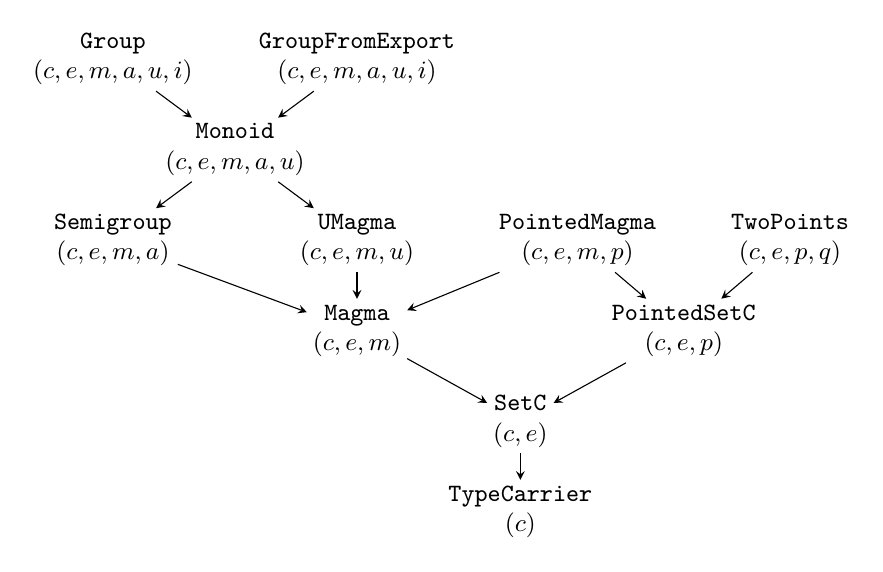
\begin{tikzpicture}[
  bundle/.style={align=center,font=\small,inner sep=2pt},
  parent/.style={->,>=stealth}]
  \node[bundle] (group) at (-0.8,4.6)
    {\ttt{Group}\\$(c,e,m,a,u,i)$};
  \node[bundle] (assembled) at (2.3,4.6)
    {\ttt{GroupFromExport}\\$(c,e,m,a,u,i)$};
  \node[bundle] (monoid) at (0.75,3.45)
    {\ttt{Monoid}\\$(c,e,m,a,u)$};
  \node[bundle] (semigroup) at (-0.8,2.3)
    {\ttt{Semigroup}\\$(c,e,m,a)$};
  \node[bundle] (unital) at (2.3,2.3)
    {\ttt{UMagma}\\$(c,e,m,u)$};
  \node[bundle] (pointed) at (5.1,2.3)
    {\ttt{PointedMagma}\\$(c,e,m,p)$};
  \node[bundle] (two) at (7.8,2.3)
    {\ttt{TwoPoints}\\$(c,e,p,q)$};
  \node[bundle] (magma) at (2.3,1.15)
    {\ttt{Magma}\\$(c,e,m)$};
  \node[bundle] (pset) at (6.45,1.15)
    {\ttt{PointedSetC}\\$(c,e,p)$};
  \node[bundle] (set) at (4.375,0)
    {\ttt{SetC}\\$(c,e)$};
  \node[bundle] (base) at (4.375,-1.15)
    {\ttt{TypeCarrier}\\$(c)$};
  \foreach \child/\ancestor in {
    group/monoid,assembled/monoid,monoid/semigroup,monoid/unital,
    semigroup/magma,unital/magma,pointed/magma,pointed/pset,
    two/pset,magma/set,pset/set}
    \draw[parent] (\child) -- (\ancestor);
  \draw[parent] (set) -- (base);
\end{tikzpicture}
\caption{The algebra structures. Solid arrows project to direct structure
parents. The generated root projects to \ttt{Type}.}
\label{fig:magma}
\end{figure}
\paragraph{Constructors and projections.}
Write $L_S$ for the ordered tuple printed under node $S$ in
Figure~\ref{fig:magma}. These tuples can be derived successively:
\[
\begin{aligned}
 (c)&\xrightarrow{+e(c)} (c,e)
     \xrightarrow{+m(c,e)} (c,e,m),\\
 (c,e)&\xrightarrow{+p(c)}(c,e,p)
     \xrightarrow{+q(c)}(c,e,p,q),\\
 (c,e,m)\cup(c,e,p)&\longmapsto(c,e,m,p),\\
 (c,e,m)&\xrightarrow{+a(c,e,m)}(c,e,m,a),\\
 (c,e,m)&\xrightarrow{+u(c,e,m)}(c,e,m,u),\\
 (c,e,m,a)\cup(c,e,m,u)&\longmapsto(c,e,m,a,u).
\end{aligned}
\]
Each $+$ applies \ruse{WF-Omit} to the displayed argument tuple and
appends the named component. The two unions use
\ruse{Parent-Union} and \ruse{Struct-Pack}: emit ready shared keys first,
then the first parent's remaining keys, then the second's.
For each structure node, $L_S=(k_1,\ldots,k_n)$ specifies the record fields,
constructor arguments and projection equations
\[
  \ttt{Make}S(x_{k_1},\ldots,x_{k_n}):S,\qquad
  \pi^S_k(\ttt{Make}S(\bar x))\equiv x_k \quad(k\in L_S).
\]
The type of $x_k$ is its descriptor evaluated at the preceding arguments.

A bare export of \ttt{Monoid} fixes $(c,e,m)$, the keys common to
\ttt{Semigroup} and \ttt{UMagma}. It takes three fixed inputs.
Writing \ttt{[Magma]} takes one packed input with the same three
projections. Writing \ttt{[]} fixes none: expansion binds
$c:\mathsf{Type}$ as an ordinary value, then uses that same $c$
in the witnesses $e,m,a,u$.

The carrier-only export \ttt{HasMonoid} stores all four non-carrier
components. We derive the other two interfaces from the same layout.

\paragraph{Fixing the magma.}
The layout $A=(c,e,m,a,u)$ follows from \ruse{Parent-Union} and \ruse{Struct-Pack}.
For $M:\ttt{Magma}$ write $(c_M,e_M,m_M)$ for its projections.
In particular $m_M$ is the entire \ttt{HasMagma} witness, including
respectfulness. Write
\[
 \mathcal A(M)=\ttt{@IsSemigroup}\;c_M\;e_M\;m_M,\qquad
 \mathcal U(M)=\ttt{@HasUnit}\;c_M\;e_M\;m_M .
\]
A value of $\mathcal U(M)$ selects the unit element \emph{and} supplies
its two laws for $m_M$. The following are the two applications of
\ruse{Export-Fix}. Here $C$ comes from the base, $F$ lists additional fixed keys and $R$ lists the remaining fields.
\[
\begin{array}{l@{\quad}l@{\quad}l@{\quad}l}
 \text{selection}&C&F&R\\
 \ttt{[Magma]} &(c,e,m)&()&(a,u)\\
 \ttt{[hasUnit, Magma]} &(c,e,m)&(u)&(a)
\end{array}
\]
In the second row, closing $u$ adds only keys already supplied by $M$.
The parameter for $M$ precedes $U:\mathcal U(M)$ even though
\ttt{hasUnit} appears first in the source selection. By
\ruse{Export-Form}, the classes have the following field telescopes
\[
\begin{aligned}
 \ttt{IsMonoid}(M)
   &\longmapsto (a:\mathcal A(M),\ u:\mathcal U(M)),\\
 \ttt{IsMonoidWithUnit}(M,U)
   &\longmapsto (a:\mathcal A(M)).
\end{aligned}
\]
For a child mixin with parameter $M:\ttt{Magma}$, the parent
\ttt{extends IsMonoid M} contributes two witnesses,
$a:\mathcal A(M)$ and $u:\mathcal U(M)$. For a child structure with
the same parameter, \ttt{with laws : IsMonoid [M]} reuses or adds
the same two components by \ruse{With-Assembly}. The assembled
\ttt{laws} view applies the constructor of \ttt{IsMonoid} to $M,a,u$.
Fixing $U$ as well leaves only $a$ to inherit or assemble.

\paragraph{Reading and rebuilding a monoid.}
Write $B(s)=\ttt{MonoidToMagma}\;s$ and
$U(s)=\ttt{Monoid\_hasUnit}\;s$. For $s:\ttt{Monoid}$,
\ruse{Parent-To} gives $B(s)$, and \ruse{Export-To} gives
\[
\begin{aligned}
 \ttt{MonoidToIsMonoid}\;s &: \ttt{IsMonoid}(B(s)),\\
 \ttt{MonoidToIsMonoidWithUnit}\;s
     &: \ttt{IsMonoidWithUnit}(B(s),U(s)).
\end{aligned}
\]
Reassembly takes the appropriate interface witness after its fixed
arguments. For $i:\ttt{IsMonoid}(M)$ and
$j:\ttt{IsMonoidWithUnit}(M,U)$ the resulting constructor tuples are
\[
 (c_M,e_M,m_M,i.a,i.u)
 \qquad\hbox{and}\qquad
 (c_M,e_M,m_M,j.a,U).
\]
Both multiplication projections reduce to $m_M$, and the second unit
projection reduces to the supplied $U$ including its law witnesses.
Reassembling an arbitrary monoid after extraction gives back the
original record by record elimination.

\paragraph{Extending the monoid.}
The next mixin, \ttt{HasInverse}, takes ordinary
parameter $A$ and parent \ttt{HasMonoid A}. The carrier-only export is
a composable mixin, so this parent expands to the four witnesses
$e,m,a,u$. An inverse law can now mention both the selected
multiplication and the selected unit. Two declarations use this interface:
\begin{verbatim}
Minks.Struct Group
  extends Monoid
  with  hasInverse : HasInverse
  exports HasGroup [carrier], IsGroup [Monoid].

Minks.Struct GroupFromExport
  extends Monoid
  with  group : HasGroup.
\end{verbatim}
The first adds an inverse witness $i(c,e,m,a,u)$ and exports the resulting
layout. In the second, \ruse{With-Assembly} reuses $e,m,a,u$ from the parent,
adds the missing inverse slot and supplies the named view
\ttt{GroupFromExport\_group}. Both layouts have six physical fields,
$(c,e,m,a,u,i)$. Projecting the inverse from the assembled view of a
value built with \ttt{GroupFromExportOfMonoid} reduces to the supplied
inverse witness.

\paragraph{All parent maps.}
Let $D$ be the solid child--parent edges of Figure~\ref{fig:magma},
and $D^+$ their nonempty transitive closure. For an ordered key list
$L$, write $s|_L=(\pi^S_k(s))_{k\in L}$. The complete families of
declared parent maps for these ten structures are indexed by
\[
\begin{aligned}
 (S,H)\in D^+:\quad &S\ttt{To}H(s)=\make_H(s|_{L_H}),\\
 (S,H)\in D:\quad &S\ttt{Of}H(h,\bar z)=\make_S((v_k)_{k\in L_S}),\\
 &v_k=\begin{cases}\pi^H_k(h)&k\in L_H,\\z_k&k\in L_S\setminus L_H.\end{cases}
\end{aligned}
\]
The missing arguments $\bar z$ follow $L_S$ order. Including the edge to the generated root yields 35
\ttt{To} maps and 12 \ttt{Of} maps; the native base contributes the
separate carrier projection. For example, the two packers of
\ttt{PointedMagma} take $(\ttt{Magma},p)$ or $(\ttt{PointedSetC},m)$.
Those of \ttt{Monoid} take $(\ttt{Semigroup},u)$ or $(\ttt{UMagma},a)$.
Both composites from \ttt{Monoid} to \ttt{Magma} construct
$\make_{\ttt{Magma}}(s|_{(c,e,m)})$ on the open input $s$.

\paragraph{Exports and registrations.}
The five actual exports can likewise be indexed by their fixed argument
tuple $\theta$ and ordered remainder $R$. Here $M$ and $N$ denote packed
magma and monoid inputs, and $u_M$ is a unit on $M$.
\[
\begin{array}{llll}
 S&E&\theta&R\\ \hline
 \ttt{Monoid}&\ttt{HasMonoid}&c&(e,m,a,u)\\
 &\ttt{IsMonoid}&M&(a,u)\\
 &\ttt{IsMonoidWithUnit}&(M,u_M)&(a)\\
 \ttt{Group}&\ttt{HasGroup}&c&(e,m,a,u,i)\\
 &\ttt{IsGroup}&N&(i)
\end{array}
\]
Each row generates the class $E(\theta)$ and constructor, the keyed
virtual mixin $R$ over $\theta$, and the maps $S\ttt{To}E$ and
$S\ttt{Of}E$ of Section~\ref{sec:relative}. Among the field-key exports,
$\ttt{HasGroup}(c)\to\ttt{HasMonoid}(c)$ drops $i$.
Including the generated root, among the eleven packed layouts, every strict inclusion already has a
declared ancestor view. The two group layouts are equal, so neither
adds a strict-containment view to the other.

\ruse{Coerce-Parent} requests the direct edges and the marked carrier
projections. For each structure row, \ruse{Inst-Field} selects every
witness key of unique class head at priority 1. Thus \ttt{TwoPoints}
registers $e$ and leaves $p,q$ explicit. For the five exports every
key in $R$ has unique class head in its source layout, so its
projection is eligible as both instance and coercion.
\ruse{Canon-View} selects all pairs in $D^+$ except
$(\ttt{TwoPoints},\ttt{PointedSetC})$: the latter parent registered
its unique \ttt{HasPoint} projection. Its direct coercion remains
eligible. Final registration is checked in the visible Rocq environment.

\subsection{A cartesian functor with fixed endpoints}
Fix cartesian categories $C,D$. A functor $F:C\to D$ preserves finite
products when it sends the chosen terminal object and binary product
cones of $C$ to terminal and product cones in $D$. Write \ttt{IsCartF F (hasTerminal C) (hasProduct C)} for this witness type. Take a mixin
$\ttt{CartLaw}(C,D,F)$ with one field of this type. Its three arguments
are ordinary parameters. Its body holds just the preservation evidence.

\begin{verbatim}
Minks.Struct FctBase (C D : CartCat)
  extends Fct C D.
Minks.Struct Packed (C D : CartCat)
  extends FctBase C D
  with law : CartLaw [C, D, carrier]
  exports CartOn [FctBase].
\end{verbatim}
The generated parent \ttt{FctCarrier C D} gives \ttt{FctBase} one field at key
\ttt{carrier}. Both structures have $\Delta=(C,D:\ttt{CartCat})$.
Writing $F$ for the value at that key, their layouts at $C,D$ are
\[
\begin{aligned}
 A_{\ttt{FctBase}} &= (F:\ttt{Fct}\ C\ D),\\
 A_{\ttt{Packed}}  &= (F:\ttt{Fct}\ C\ D,\quad
                       \ttt{law}:\ttt{CartLaw}(C,D,F)).
\end{aligned}
\]
Thus $\ttt{MakePacked}\ C\ D$ takes $F$ once, followed by a witness
for that very $F$. For $p:\ttt{Packed}\ C\ D$, write $\pi(p)$ for its
view in $\ttt{FctBase}\ C\ D$. The parent's functor projection on
$\pi(p)$ reduces to the functor projection on $p$.

Fix $b:\ttt{FctBase}\ C\ D$ with functor $F_b$.
Then $\ttt{CartOn}\ C\ D\ b$ has the single field of type
$\ttt{CartLaw}(C,D,F_b)$. Extracting from $p$ therefore has type
$\ttt{CartOn}\ C\ D\ \pi(p)$ and its field reduces to the law of $p$.
Conversely, packing $b$ and an export witness uses $F_b$ and the law
stored in that witness. Both projections reduce to the supplied values on open inputs.

\subsection{Scope and rejection cases}
\paragraph{Explicit and inferred inputs.}
The mixin \ttt{FlagPair} takes two ordinary \ttt{HasFlag} values.
\begin{verbatim}
Minks.Struct PairAt (p q : HasFlag)
  with  seed : HasFlag,
        chosen : FlagPair [p, q],
        mixed : FlagPair [seed, p].

Minks.Struct Diagonal (x : HasFlag)
  extends PairAt x x.
\end{verbatim}
Immediately after \ttt{seed}, an omitted list for \ttt{FlagPair}
selects $[\ttt{seed},\ttt{seed}]$. The formals $p,q$ remain in scope
and are available explicitly. Before \ttt{seed} the same omission fails.
With two distinct flag fields, it is ambiguous. In the child,
\ttt{chosen} has arguments $[x,x]$ and \ttt{mixed} has
$[\ttt{seed},x]$. Thus in context $x:\ttt{HasFlag}$ the parent view has
type $\ttt{Diagonal}(x)\to\ttt{PairAt}(x,x)$. In context
$x,y:\ttt{HasFlag}$ the source still cannot supply
$\ttt{PairAt}(x,y)$: the descriptors of \ttt{chosen} disagree.
Substitution acts on resolved references. The parent view copies the three projections, so its \ttt{chosen}
and \ttt{mixed} projections reduce to those of the child on an open input.

For discovery, take an independent structure with the layout of
$\ttt{PairAt}(x,x)$ and one extra key. Matching \ttt{chosen} gives
$B=\{p\mapsto x,q\mapsto x\}$, and \ttt{mixed} confirms the binding of
$p$. This yields a view to $\ttt{PairAt}(x,x)$. If the target also
has an ordinary parameter $z$ absent from all descriptors, $B$ has
no entry for $z$. Discovery skips the view even if only one source
parameter has the right type. A declared parent can supply $z$.

\paragraph{Conflict and ambiguity.}
Suppose one parent supplies $m:\mathit{HasMagma}(c,e_1)$ and
another supplies $m:\mathit{HasMagma}(c,e_2)$ with $e_1\ne e_2$ as
keys. The union fails at $m$, even if the equivalence terms happen
to compute alike. Keeping two keys $m_1,m_2$ on the \emph{same}
$c,e$ makes both available. A subsequent associativity component
with omitted arguments then has two candidate tuples. Specifying
$[c,e,m_1]$ resolves it. The two multiplication projections remain
available as explicit selections.

\paragraph{Complete and partial assembly.}
Fix a carrier and an equivalence. Suppose the remainder of an interface
has two keys: $m$ for a multiplication and $a$ for its associativity
witness. The available multiplications $l,r$ have different keys from
$m$. Write $a_l,a_r$ for witnesses at $l,r$, also with fresh keys.
The table lists the complete selections and the resulting decision.
\[
\begin{array}{lll}
 \text{available fields}&\mathsf{reuse}&\text{result}\\ \hline
 l,r,a_l     &\{(l,a_l)\}         &\text{reuse both fields}\\
 l,r,a_l,a_r &\{(l,a_l),(r,a_r)\} &\text{reject two complete matches}\\
 l           &\varnothing          &\text{reuse }l,\ \text{append }a(l)\\
 l,r         &\varnothing          &\text{reject ambiguous fill}
\end{array}
\]
In the first row the branch starting with $r$ has no completion, so
the initial choice between $l$ and $r$ alone cannot decide ambiguity.

\paragraph{Names at the boundary.}
If two parents call their projection for key \ttt{op} \ttt{leftMul}
and \ttt{rightMul}, a child \ttt{Joined} inheriting both publishes
\ttt{Joined\_op}. Both parent projections still read that same field.
Separately, if a header parameter and a field key are both named
\ttt{x}, the input \ttt{[x]} is ambiguous by \ruse{Input-Name}.
Renaming the header binder to \ttt{p} makes \ttt{[p]} select the
parameter and \ttt{[x]} the field.

\paragraph{Universes and competing views.}
If two parent applications force distinct explicit annotations for
one shared witness position, the mixin merge fails. A separate
failure occurs when otherwise matching descriptors require an
unsatisfiable host constraint such as $v<v$. Distinct components can
also yield distinct explicit maps to a smaller interface. If the
key-preference rules leave two matches for one inferred assembly,
inference fails. If two separately registered coercions to the same
target select different components, their paths require a host
conversion check. Existence of both typed maps does not imply that
check succeeds.

\begin{thebibliography}{9}
\bibitem{hb}
Cyril Cohen, Kazuhiko Sakaguchi, and Enrico Tassi.
\emph{Hierarchy Builder: Algebraic Hierarchies Made Easy in Coq with Elpi
(System Description)}.
FSCD 2020, LIPIcs 167, article 34.
\href{https://doi.org/10.4230/LIPIcs.FSCD.2020.34}{DOI 10.4230/LIPIcs.FSCD.2020.34}.

\bibitem{validating}
Kazuhiko Sakaguchi.
\emph{Validating Mathematical Structures}.
IJCAR 2020, LNCS 12167, pp.~138--157.
\href{https://doi.org/10.1007/978-3-030-51054-1_8}{DOI 10.1007/978-3-030-51054-1\_8}.
\href{https://pmc.ncbi.nlm.nih.gov/articles/PMC7324068/}{Open text}.
\end{thebibliography}
\end{document}
